\section{}

Da das Intervall $[-1,1]$ symmetrisch um $0$ ist, sind die Unterräume $U, G \subseteq C[-1, 1]$ der ungeraden und geraden Funktionen orthogonal bezüglich des $L^2$-Skalarproduktes.
Da die Polynome $x^i$ alle gerade oder ungerade sind (abhängig von der Parität von $i$) sind somit auch alle Legendre-Polynome gerade oder ungerade.
Da die Runge-Funktion gerade ist, genügt es für die Approximation dabei, die geraden Legendre-Polynome zu betrachten;
dies sind gerade die Legendre-Polynome von geraden Grad (denn $x^i$ ist genau dann gerade, wenn $i$ gerade ist).

Wir nutzen nun den folgenden Code, um die Liste der ersten $n$ Approximationen zu bestimmen:

\lstinputlisting[style=pythoncode, firstline = 1, lastline = 30]{chapter_09/exercise_09_49.py}

Wir testen die Approximationen für die bekannten Werte $n = 5, 11, 17$:

\lstinputlisting[style=pythoncode, firstline = 34, lastline = 43]{chapter_09/exercise_09_49.py}

Hierdurch ergeben sich für die Approximationen die folgenden Graphen:



\subsection{}

\begin{center}
  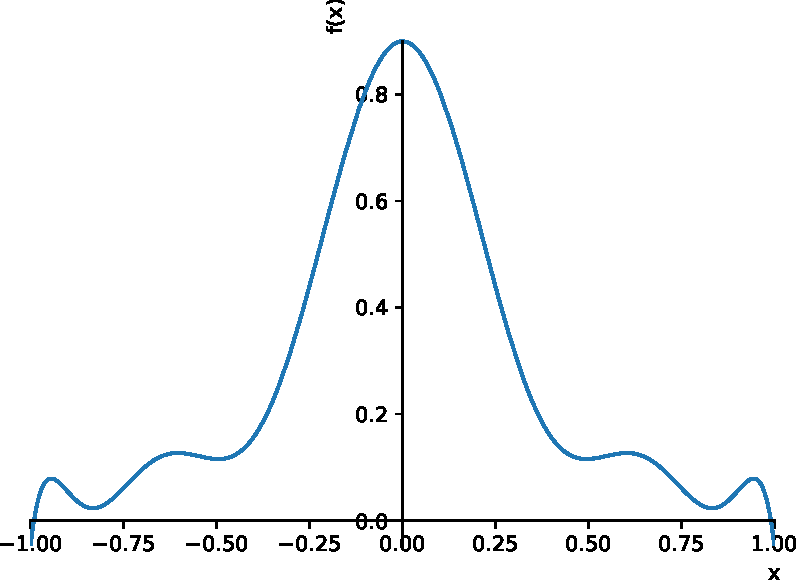
\includegraphics[width = 0.3\textwidth]{chapter_09/exercise_09_49_figure_1.pdf}
  \hspace{1em}
  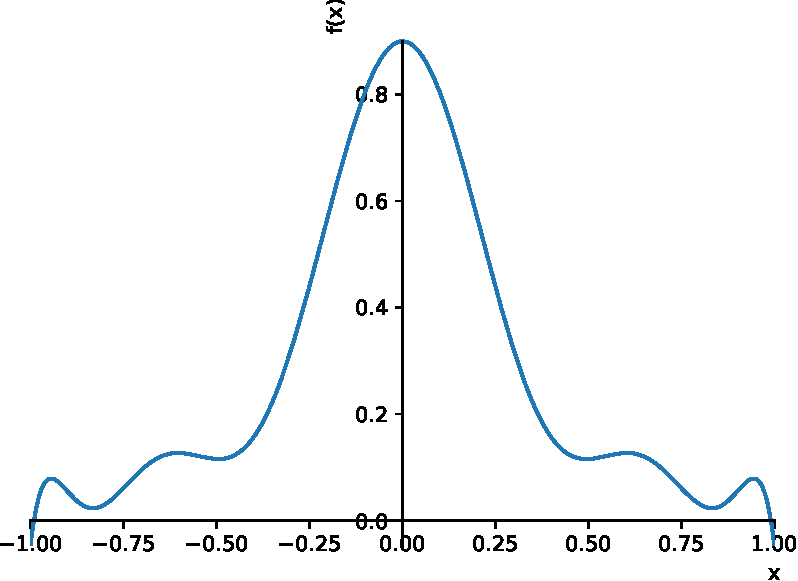
\includegraphics[width = 0.3\textwidth]{chapter_09/exercise_09_49_figure_2.pdf}
  \hspace{1em}
  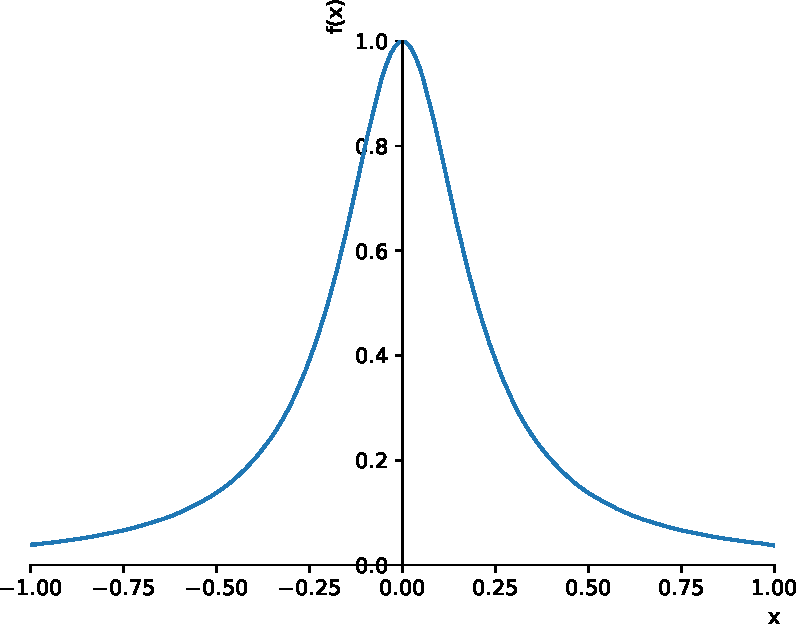
\includegraphics[width = 0.3\textwidth]{chapter_09/exercise_09_49_figure_3.pdf}
\end{center}



\subsection{}

Die Fehler sind entsprechend klein:

\begin{center}
  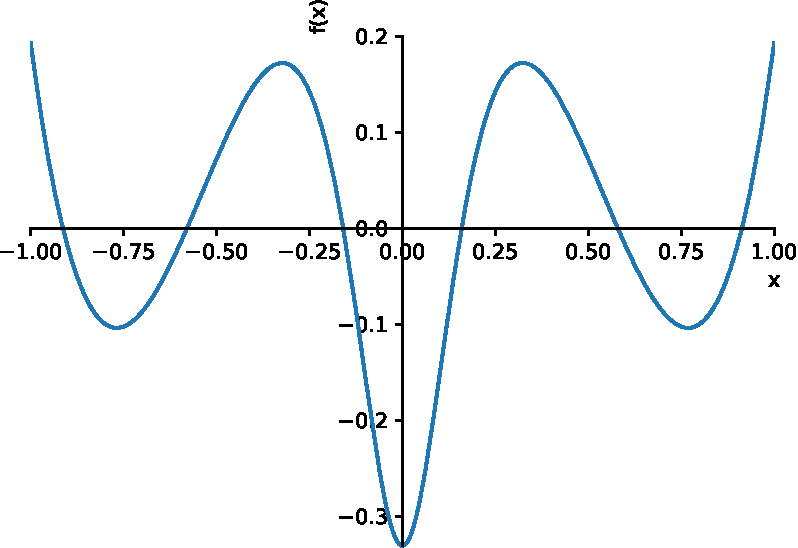
\includegraphics[width = 0.3\textwidth]{chapter_09/exercise_09_49_figure_4.pdf}
  \hspace{1em}
  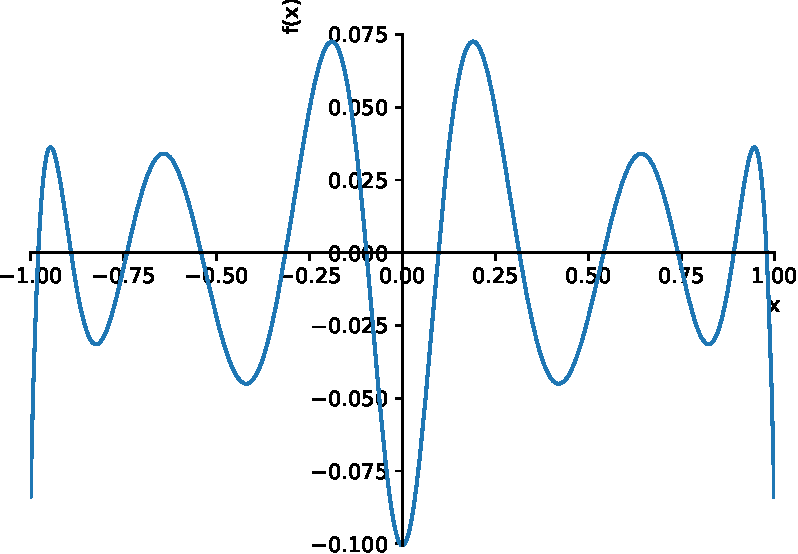
\includegraphics[width = 0.3\textwidth]{chapter_09/exercise_09_49_figure_5.pdf}
  \hspace{1em}
  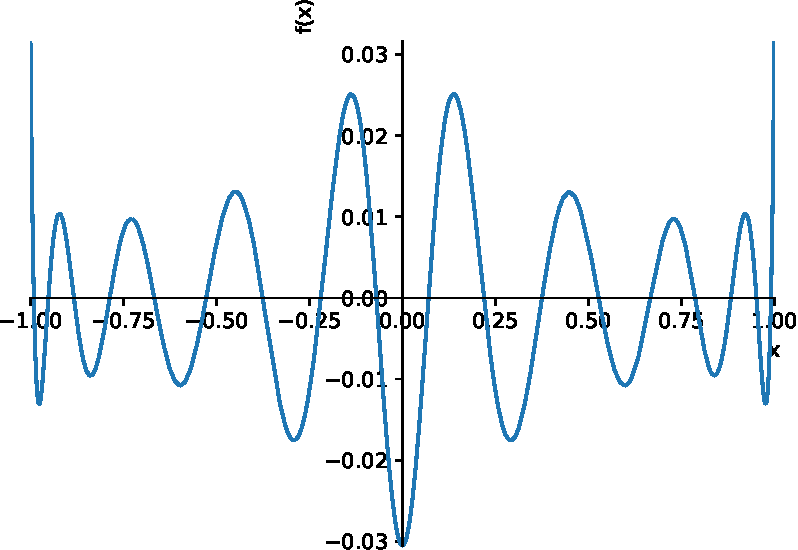
\includegraphics[width = 0.3\textwidth]{chapter_09/exercise_09_49_figure_6.pdf}
\end{center}



